% sensingHardware.tex
\subsubsection{MQ6 Liquid Petroleum Gas Sensor}
\par The MQ-6 LPG Sensor is a highly sensitive, metal oxide based detector\cite{Dey}, designed to detect different petroleum derived gases, such as propane, butane and other flammable gasses including natural gas and methane. The sensor's conductivity changes proportional to the gas concentration in contact with the Tin Dioxide (SnO\textsubscript{2}) sensing material within the shroud of the unit. The relatively low cost and wide range of detection make it an excellent choice for our system. The MQ-6 sensor operates at 5-volts.
\begin{figure}[h!]
	\centering
	\begin{subfigure}[t]{0.22\textwidth}
		\centering
		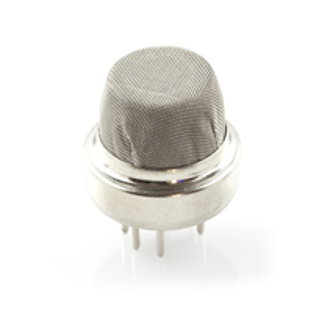
\includegraphics[width=.8\textwidth]{mq6.png}
		\caption{MQ6 Liquid Petroleum Gas Sensor Package}
	\end{subfigure}
	\begin{subfigure}[t]{0.22\textwidth}
		\centering
		\includegraphics[width=\textwidth]{mq6diag.png}
		\caption{MQ6 Liquid Petroleum Gas Sensor Diagram}
	\end{subfigure}
	\caption{MQ6 Gas Sensor}
\end{figure}
\subsubsection{Parallax Passive Infra-red Motion Sensor}
\par To trigger subsequent elements of the proposed system we needed a motion detecting sensor. An infra red motion sensor works through applying the concept of pyroelectricity, a characteristic of materials that will generate a potential difference when heated. In this case the heat source is reflected infra red light. When there is no movement, current through a resistor in series with the pyroelectric material's electrodes will be constant. When movement occurs in the field of view of the infra red source, the amount of reflected light will change causing a change in the pyroelectric voltage. This change in voltage causes the current through the circuit to change, this is measured triggers the output accordingly.\cite{Webster}
\begin{figure}[h]
	\centering
	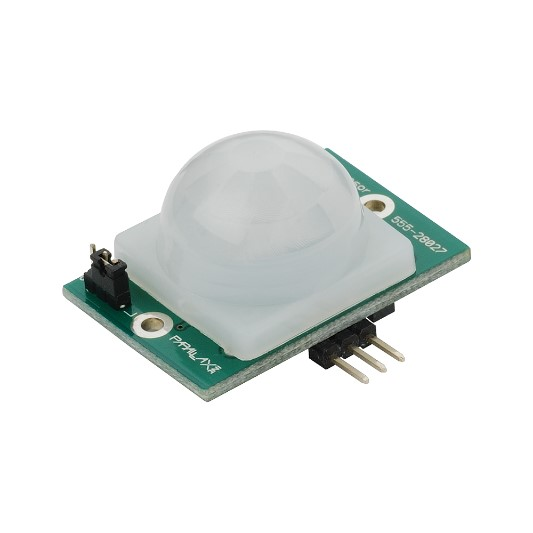
\includegraphics{pirDevice.jpg}
	\caption{PIR Motion Sensing Module}
\end{figure}
\newpage
\par In our case, we desire a sensor such that negligible movement will be ignored. If this input was to trigger a camera, picking up a very small object's movement or similar "false alarms" would result in an over abundance of images taking up memory on the users pc or the system itself. Moreover if this device triggered an alarm, false alarms would be unacceptable in most cases. Most infra-red motion sensors on the market today are all-in-one units that take this into consideration by only raising a digital output high when a sufficiently large current change in the pyroelectric circuit is measured by the sensor module. 
\par For our system we chose to use a Parallax passive infra-red \textit{(PIR)} motion sensor. This PIR motion sensor operates from 3 volts to 6 volts meaning it can utilize the same power source as the XBee modules. The XBee will read the digital signal generated by the PIR sensor to trigger the rest of the system remotely.
